%% ====================================================================
%%  ACT III: STRUCTURAL EXTENSIONS (~5pp)
%% ====================================================================
\section{Structural Extensions: Depth, Cost, and Transfer}
\label{sec:extensions}

The four-term decomposition tells a builder which lever matters.
This section shows how to pull the depth lever (graph-depth model and crossover theorem) and when to reuse what was learned (transfer theory).

\subsection{From Four Terms to Depth: The Connective Step}
\label{sec:connective}

% W3: Connective paragraph verifying P_D satisfies packed-family structure
The four-term decomposition (Theorem~\ref{thm:four-term}) applies to any model~$M$ operating within the packed-family framework.
To extend it to depth-$D$ designs---where an agent makes $D$ independent sequential attempts---we must verify that the boosted success probability $P_D(s, M) = 1 - (1 - p(s,M))^D$ preserves the packed-family structure.

It does.
Conditional on mode~$s$, the minimum of $D$ independent geometric random variables is itself geometric with parameter~$P_D(s, M)$.
The mode distribution~$\pi$ does not change (it is a property of the task, not the agent).
The cost becomes $D \cdot \kappa(M)$ per instance.
Therefore, the four-term decomposition applies to depth-$D$ designs with $p(s,M)$ replaced by $P_D(s,M)$ and $\kappa(M)$ replaced by $D \cdot \kappa(M)$, and all four terms remain independently estimable.

\subsection{The Graph-Depth Model}
\label{sec:graph-depth}

% SOURCE_CLAIM: C52
\begin{definition}[Graph-depth extension]
\label{def:graph-depth}
Given a packed latent-mode family with mode distribution~$\pi$, model~$M$ with per-attempt cost~$\kappa(M)$ and per-mode success probabilities~$p(s,M)$, the \emph{$D$-depth extension} makes $D \ge 1$ independent sequential attempts.
The success probability on mode~$s$ is $P_D(s,M) = 1 - r_s^D$ where $r_s = 1 - p(s,M)$.
The expected log certified time is $L(M, D) = \sum_s \pi_s (-\log(1 - r_s^D))$.
\end{definition}

\begin{remark}[Independence caveat]
\label{rem:independence}
The independent-attempts model is a simplifying assumption.
Real orchestration steps exhibit inter-step dependence: later steps condition on earlier failures, use different prompts, or exploit partial progress.
Independence provides a conservative estimate of depth benefits---dependent attempts with information reuse can only improve upon it.
\end{remark}

The builder's problem is to choose $D$ to minimize expected log certified time subject to a cost budget:

% SOURCE_CLAIM: C53
\begin{theorem}[Optimal depth and monotonicity]
\label{thm:optimal-depth}
Under the packed-family model with geometric trials, exogenous mode distribution, monotone competence, continuous relaxation of~$D$, and interior solution ($\mu > 0$):
\begin{enumerate}[label=(\alph*)]
  \item The optimal depth $\Dstar(M)$ is the unique solution to $F(\Dstar; M) = \mu \cdot \kappa(M)$, where $F(D; M) = \sum_s \pi_s r_s^D (-\log r_s) / (1 - r_s^D)$.
  \item $F$ is strictly decreasing in~$D$, so $\Dstar$ is unique.
  \item $d\Dstar / dt_0 < 0$: a more competent model requires fewer orchestration steps.
  \item $d\Dstar / d(\kappabig/\kappa(M)) > 0$: a cheaper model (relative to alternatives) affords more steps.
\end{enumerate}
\end{theorem}

\begin{proof}[Proof sketch]
Differentiate $L(M,D) + \mu D \kappa$ to obtain the FOC.
Uniqueness follows from $dF/dD < 0$, proved by showing each summand has negative derivative via $-r_s^D (\log r_s)^2 / (1-r_s^D)^2 < 0$.
Monotonicity in competence uses the implicit function theorem: the auxiliary function $h(r) = -D\log r - 1 + r^D$ satisfies $h(1) = 0$ and $h'(r) < 0$ on $(0,1)$, giving $dg/dr > 0$.
Full proof in \appref{app:graph-depth}.
\end{proof}

The qualitative intuition is straightforward: stronger models need simpler architectures.
The contribution is making this a theorem with explicit conditions and a computable characterization.
Numerical validation confirms the FOC is exact to~$0.001$ across 50~scenarios, with zero monotonicity violations in 1{,}000 parameter combinations.

\subsection{The Crossover Theorem}
\label{sec:crossover}

One might expect model capability to be the dominant design variable---this is the implicit assumption behind benchmark racing.
The crossover formula reveals otherwise: in the cost-adjusted regime, the ratio of per-step costs often determines which model wins, regardless of the competence gap.

% SOURCE_CLAIM: C54
\begin{theorem}[Crossover: when small-model-big-graph dominates]
\label{thm:crossover}
Given two models $M_s$ (small, cheap) and $M_l$ (large, expensive) with $\kappa(M_l) > \kappa(M_s)$ and $p(s, M_l) > p(s, M_s)$ for all modes~$s$:
\begin{enumerate}[label=(\alph*)]
  \item There exists a finite crossover depth $\Dcross \ge 1$ such that $L(M_s, \Dcross) = L(M_l, 1)$.
  \item For a single mode: $\Dcross = \log(1 - p_l) / \log(1 - p_s)$.
  \item For multiple modes: $\Dcross$ is the unique solution to $\sum_s \pi_s (-\log(1 - r_s(M_s)^D)) = \sum_s \pi_s (-\log p(s, M_l))$.
  \item For hard tasks, the hardest-mode formula $\hat{D} = \max_s \log r_l(s) / \log r_s(s)$ provides a practical estimate of~$\Dcross$. Empirically, $\hat{D} \ge \Dcross$ in all 50~tested parameter settings (mean overestimate $1.8\times$, max $3.9\times$). We conjecture $\hat{D} \ge \Dcross$ in general; a proof is open.
  \item The small model with $\Dcross$ attempts dominates at equal cost if and only if $\Dcross \le \kappa(M_l) / \kappa(M_s)$.
\end{enumerate}
\end{theorem}

At current large-model pricing (roughly $10\times$ more expensive than small models), the small model with retries wins for any task where $\Dcross \le 10$---which covers most practical scenarios where per-mode success probabilities differ by less than an order of magnitude.

% SOURCE_CLAIM: C55
\begin{corollary}[Comparative statics]
\label{cor:crossover-statics}
$\Dcross$ is increasing in the competence ratio $p_l/p_s$.
The cost-adjusted condition $\Dcross \le R$ is more easily satisfied when: (i)~$R$ is large (cheap model relative to expensive); (ii)~the competence ratio is moderate; (iii)~the task is specialist ($\Meff$ small), because the hardest mode dominates.
\end{corollary}

Numerical validation confirms: the single-mode formula is exact to~$0.004$ across 100~pairs; the cost-adjusted condition correctly predicts 99\% of 200~scenarios.
The hardest-mode estimate is tighter for specialist tasks ($\Meff$ small) and looser for generalist distributions.

\paragraph{Worked example.}
Consider two models: a small model with $p_s = 0.2$ per attempt at cost $\kappa_s = 1$, and a large model with $p_l = 0.6$ per attempt at cost $\kappa_l = 10$.
The crossover depth is $\Dcross = \log(0.4)/\log(0.8) \approx 4.1$.
Since $\Dcross = 4.1 < 10 = R$, the small model with 4--5 attempts dominates the large model with one attempt at equal cost.
The small model achieves success probability $1 - 0.8^5 = 0.67$ for cost~$5$, compared to the large model's $0.6$ for cost~$10$.

\subsection{Transfer Theory}
\label{sec:transfer}

% W4: Transfer theory 4-paragraph structure, no "prove"/"theorem"

The prior framework~\citep{beneventano2026framework} establishes two formal notions of task equivalence for agent design.
\emph{Post-training equivalence} holds when two task distributions produce the same competence profile $\{p(s,M)\}_s$ for all models~$M$: the same models are good at the same things.
\emph{Orchestration equivalence} holds when the optimal routing policy is the same: the same workflow applies.

These notions are independent: a pair of tasks can share identical competence profiles while requiring entirely different routing policies, or vice versa.
The formal infrastructure for this independence is established in the prior work; constructive examples remain future work.

This independence yields a three-case decision rule for when agent-system results transfer to a new task domain.
Consider a practitioner who has optimized an agent system for Lean theorem proving and now faces a code-repair task distribution, using two models at cost ratios varying across $\{2, 10, 50\}$.
\emph{Plug-and-play}: at cost ratio~$2$, if both tasks have similar mode structure and the same model is relatively better on each mode, the full design transfers---models, routing, depth, everything.
\emph{Re-route}: at cost ratio~$10$, if the models are equally capable on the new domain but the task distribution differs (different relative frequencies of modes), the routing policy must be rebuilt from new pilot data, but the model selection stands.
\emph{Start over}: at cost ratio~$50$, if the cheap model dominates on every mode of the new domain (routing is trivial by the condition in \secref{sec:routing-triviality}), the expensive model is abandoned entirely and the optimization must restart.

Formal quantitative treatment---including constructive independence examples, estimation protocols for the transfer decision, and error bounds---is future work.

% W5: Transfer trichotomy 2-axis figure description
\begin{figure}[t]
  \centering
  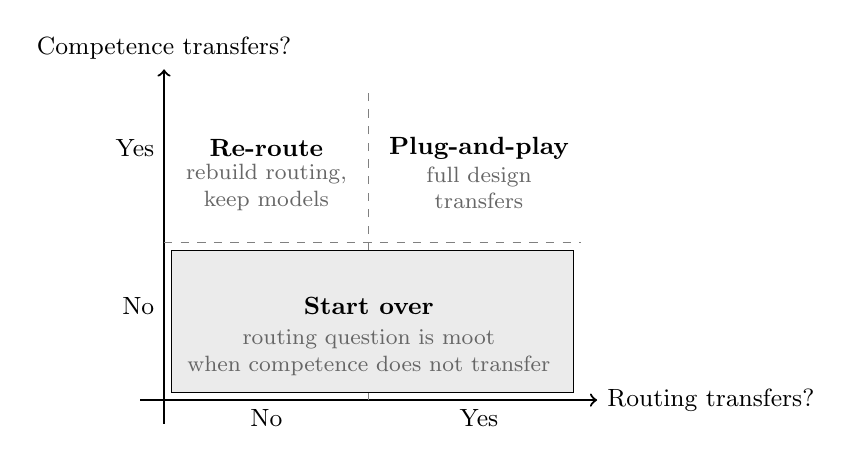
\begin{tikzpicture}[scale=1.0]
    % Axes
    \draw[->, thick] (-0.3,0) -- (5.5,0) node[right] {\small Routing transfers?};
    \draw[->, thick] (0,-0.3) -- (0,4.2) node[above] {\small Competence transfers?};
    % Labels
    \node at (1.3,0) [below] {\small No};
    \node at (4.0,0) [below] {\small Yes};
    \node at (0,1.2) [left] {\small No};
    \node at (0,3.2) [left] {\small Yes};
    % Grid lines
    \draw[dashed, gray] (2.6,0) -- (2.6,4.0);
    \draw[dashed, gray] (0,2.0) -- (5.3,2.0);
    % Quadrants
    \node[align=center, font=\small\bfseries] at (1.3,3.2) {Re-route};
    \node[align=center, font=\footnotesize, text=black!60] at (1.3,2.7) {rebuild routing,\\keep models};
    \node[align=center, font=\small\bfseries] at (4.0,3.2) {Plug-and-play};
    \node[align=center, font=\footnotesize, text=black!60] at (4.0,2.7) {full design\\transfers};
    % Lower region (merged)
    \draw[fill=black!8] (0.1,0.1) rectangle (5.2,1.9);
    \node[align=center, font=\small\bfseries] at (2.6,1.2) {Start over};
    \node[align=center, font=\footnotesize, text=black!60] at (2.6,0.6) {routing question is moot\\when competence does not transfer};
  \end{tikzpicture}
  \caption{The transfer trichotomy.
  Two binary questions---does the competence profile transfer, and does the routing policy transfer?---yield three named cases for reusing agent design results across task domains.
  The lower region collapses because when competence does not transfer, the routing question is moot.}
  \label{fig:transfer-trichotomy}
\end{figure}
